\documentclass[a4paper, 11pt,reqno]{article}
\input{/Users/olivierglorieux/Desktop/BCPST/2020:2021/preambule.tex}
\newif\ifshow
\showtrue
\input{/Users/olivierglorieux/Desktop/BCPST/2021:2022/ifshow.tex}
\newcommand{\jour}[1]{
\begin{center}
\underline{\textbf{#1}}
\end{center}

 }

\author{Olivier Glorieux}


\begin{document}

\title{Devoir Vacances
}

\begin{center}
\underline{\textbf{Lundi 24/10/2021}}
\end{center}

\begin{correction}
\begin{enumerate}
\item $D_f= \R^*$, $f'(x) = (2x +1) e^{-\frac{1}{x}}$
\item $z=\frac{-1}{2^6}$, $Re(z) =\frac{-1}{2^6}$, $Im(z)=0$
\item $\frac{(n+3)(n+4)}{2} - 1$
\item $u_n= -\frac{1}{2^n} +2$
\end{enumerate}
\end{correction} 







\jour{Mardi 25/10/2021}
\begin{correction}
\begin{enumerate}
\item $D_f= \R$, $f'(x) =\frac{e^x+2x}{e^x+x^2}$
\item $\frac{1}{2} \left(  \left(\frac{3}{2}\right)^n -1- \frac{1}{2^n}\right)$
\item $8$
\item $u_n = 2^n\cos\left(\frac{n\pi}{3}\right)$
\item $z=e^{-i\pi/6} $ donc $Re(z) = cos(\frac{pi}{6}$ et $Im(z) =\sin(\frac{-\pi}{6}$
\end{enumerate}
\end{correction} 






\jour{Mercredi 26/10/2021}
\begin{correction}
\begin{enumerate}
\item $D_f= \R$, $f'(x) =(\cos(x) -x\sin(x) ) e^{x\cos(x)}$
\item 
Soit $S_n=\ddp \sum_{i=0}^n (2x)^{2i}$, (Remarque : $\suite{S}$ est quasiment sous la forme d'une somme d'une suite géométrique. On utilise $a^{nm} = (a^{n})^m)$) 

$$S_n = \sum_{i=0}^n ((2x)^2)^i= \sum_{i=0}^n (4x^2)^i$$
On applique ensuite la formule du cours : 
Si $x^2\neq \frac{1}{4}$:
$$S_n =\frac{1-(4x^2)^{n+1}}{1-4x^2}$$
Et donc :
$S_n= \frac{1-(4x^2)^{n+1}}{1-4x^2} = \frac{1-4^{n+1}x^{2n+2}}{1-4x^2}$ si $x^2\neq \frac{1}{4}$\\
$S_n=n+1$ si $x^2=\frac{1}{4}$

\item 
Soit $v_n =u_n-\ell$ avec $\ell \in \R$. On cherche $\ell$ afin que $\suite{v}$ soit géométrique. 

\begin{align*}
v_{n+1}&=u_{n+1}-\ell\\
			&= 2u_n+1-\ell\\
			&=2(v_n+\ell) +1-\ell\\
			&=2v_n+ \ell +1
\end{align*}
Ainsi, en prenant $\ell =-1$, on obtient $v_n = u_n+1$ qui est une suite géométrique de raison $2$. 
Donc $v_n =v_0 2^n $ et $v_0 = u_0+1=2$. On obtient donc $v_n =2^{n+1}$. En revenant à $u_n$ cela donne  : 
\conclusion{$u_n=v_n-1 = 2^{n+1}-1$}



\item $0$
\item $\cS=\{ \sqrt{2}, -\sqrt{2}\}$
\end{enumerate}
\end{correction} 


\jour{Jeudi 27/10/2021}
\begin{correction}
\begin{enumerate}
\item $D_f= \R$, $f'(x) =\frac{6\sin^2(2x)\cos(2x) (2+\cos(5x) - 5\sin^3(2x)\sin(5x)}{(2+\cos(5x))^2}$
\item On étudie $D(x) = e^x-(x+1)$, définie sur $\R$ et $D'(x) = e^x-1$. 
$D'(x) \geq 0 \equivaut x\geq 0$. Le minimum de $D$ est obtenu en $0$ et vaut $e^0-(0+1)=0$ donc 
$D(x)\geq 0$ pour tout $x\in \R$. Donc $e^x \geq x+1$
\item Soit $S_n =\ddp  \sum_{k=2}^n (k^2+1)$

\begin{align*}
S_n& =\sum_{k=2}^n k^2+\sum_{k=2}^n 1 \quad \text{ linéarité}\\
	&=\sum_{k=1}^n k^2- 1^2 + (n-1)  \quad \text{ n-1 nombre entre 2 et n}\\
	&=\frac{n(n+1)(2n+1)}{6} -1  +n-1\quad { formule du cours}
\end{align*}


\conclusion{$S_n=\frac{n(n+1)(2n+1)}{6}+ n-2$}
\item $z= \sqrt{2} e^{i\pi/2}$
\item 
\begin{lstlisting}
def somme_harmonique(n):
  S=0
  for k in range(1,n+1):
    S=S+1/k
  return(S)
\end{lstlisting}
\end{enumerate}
\end{correction} 




\jour{Vendredi 28/10/2021}
\begin{correction}
\begin{enumerate}
\item
$$f(x) = \left( \frac{\sqrt{x^2+3x}}{3^x}\right)^4$$

Rappelons que $3^x=exp(x \ln (3)) $ est définie sur $\R$ et strictectement positif. 

Donc $f$ est définie pour tout $x$ vérifiant $x^2+3x \geq 0 $ c'est à dire $x(x+3)\geq 0$ soit $D_f=]-\infty , -3]\cup [0,+\infty[$.
Et $f$ est dérivable sur $]-\infty , -3[\cup ]0,+\infty[$.

On simplifie $f$  en utilisant la puissance $4$ : on a $$f(x) = \frac{(x^2+3x)^2}{3^{4x}}.$$
Maintenant on utilise la formule de la dérivée d'un quotient $f(x) =\frac{u(x)}{v(x)}$ avec 
$u(x) = (x^2+3x)^2$ et $v(x) = 3^{4x} =\exp(4x\ln(3))$. 

Calculons les dérivées de ces deux fonctions : 

$$u'(x) = 2 (2x+3) (x^2+3x)$$ et 
$$v'(x) = 4\ln(3) \exp(4x\ln(3) ) =4\ln(3) 3^{4x} $$
On obtient alors : 
\begin{align*}
f'(x) &= \frac{u'(x)v(x) - u(x)v'(x) }{(v(x))^2}\\
&= \frac{2(2x+3)(x^2+3x)3^{4x}-(x^2+3x)^2 4\log(3) 3^{4x}}{3^{8x}}
\end{align*}


\item $0$
\item $u_n=1$
\item 0
\item 
\begin{lstlisting}
from random import randint
def lancer_de_de():
  de=randint(1,6)
  return(de)
\end{lstlisting}
\end{enumerate}
\end{correction} 
\newpage

\jour{Samedi 29/10/2021}
\begin{correction}
\begin{enumerate}
\item On étudie $D(X) =\ln(1+X) -X$ sur $\R_+$. $D(X)\leq 0 \equivaut \ln(1+X)\leq X \equivaut 1+X\leq e^X$ qui est vrai pour tout $X\in \R$ d'aprés l'ex 4.
Donc $\ln(1+X) \leq X$ pour tout $X\geq 0$. Pour tout $x\in \R$, $x^2 \geq 0$ donc 
$D(x^2) \leq 0$ c'est-à-dire $\ln(1+x^2)\leq x^2$
\item $D_f = [1,+\infty[$ et dérivable sur $]1, +\infty[$. 
$$f'(x) = \frac{1+\sqrt{x^2-1}}{x^2-1+x\sqrt{x^2-1}}$$
\item 1
\item $\cS=[\frac{1}{2}, +\infty[$
\item 
\begin{lstlisting}
from math import *
def solution(x,y,z):
  L_1= (pi**2)*x +1.4*y +z 
  L_2= log(2)*x+1.7*y +(2**4)*z
  if L_1==120 and L_2==0:
    return(True)
  else:
    return(False)
\end{lstlisting}
def solutio
\end{enumerate}
\end{correction} 

\jour{Dimanche 30/10/2021}
REPOS ! 
\jour{Lundi 31/11/2021}
REPOS ! 
\newpage
\jour{Mardi 01/11/2021}
\begin{correction}
\begin{enumerate}
\item $D_f= ]1,+\infty[$, $f'(x) = \frac{1}{x\ln(x)}$
\item $f(x) =x^x=e^{x\ln(x)}$ $D_f=]0,+\infty[$ 
$f'(x) = (1+\ln(x))e^x{x\ln(x)}$, $f'(x) \geq 0 \equivaut x\in ]e^{-1}, +\infty[$

\begin{tikzpicture}
   \tkzTabInit{$x$ / 1 , $f'(x)$ / 1, $f(x)$ / 1.5}{$0$, $e^{-1}$, $+\infty$}
   \tkzTabLine{, -, z, +, }
   \tkzTabVar{+/ 1, -/$\frac{1}{e^e}$, +/ $+\infty$}
\end{tikzpicture}
\item $u_n =\exp(\ln(2) (2^n-1)) = 2^{2^n-1}$
\item $\frac{1}{2}$
\item $z= \frac{(1+i)}{\sqrt{2}}$
\end{enumerate}
\end{correction} 

\newpage


\jour{Mercredi 02/11/2021}
\begin{correction}
\begin{enumerate}
\item $D_f =]-2,-\frac{2}{3}[ \cup ]\frac{2}{3},+\infty[$
$$f'(x) =\frac{-4-18x}{\sqrt{9x^2-4} (x+2)}$$
\item 
$\ddp \sum_{k=0}^{n-1} q^k = \frac{1-q^n}{1-q}$ pour $q\neq 1$. 

On a donc 
\begin{align*}
\sum_{k=0}^{n-1} e^{\frac{ik\pi}{n}}&=\sum_{k=0}^{n-1} \left(e^{\frac{i \pi}{n}} \right)^k\\
														&=  \frac{1-e^{\frac{i \pi}{n}^n}}{1-e^{\frac{i \pi}{n}}}\\
														&=\frac{1-e^{i \pi}}{1-e^{\frac{i \pi}{n}}}\\
														&=\frac{2}{1-e^{\frac{i \pi}{n}}}
\end{align*}
\conclusion{ $\sum_{k=0}^{n-1} e^{\frac{ik\pi}{n}} = \frac{2}{1-e^{\frac{i \pi}{n}}}$}


\begin{align*}
\prod_{k=0}^n e^{\frac{ik\pi}{n}} &=e^{\sum_{k=0}^n \frac{ik\pi}{n}}\\
													&= e^{i\pi\frac{n(n+1)}{2n}}\\
													&= e^{i\pi\frac{n+1}{2}}
\end{align*} 

\item $\frac{1}{2}\left( \frac{n(n+1)(2n+1)}{6} +n\right)$
\item \begin{lstlisting}
from random import randint
def somme_des_lancers(n):
  S=0
  for i in range(n):
    S=S+randin(1,6)
  return(S)
\end{lstlisting}
\item Notons $(E)$ l'équation $\sqrt{x+1} \leq x$.


L'ensemble de définition de l'équation est $D=[-1,+\infty[$.
Afin de mettre au carré on distingue les deux cas : 
\begin{itemize}
\item Cas 1 : $x\geq 0$.

Alors $(E) \equivaut x+1 \leq x^2 \equivaut x^2-x-1\geq 0$
On factorise $x^2-x-1$ à l'aide des racines $r_1=\frac{1-\sqrt{5}}{2}$ et $r_1=\frac{1+\sqrt{5}}{2}$, on obtient 
$$(E) \equivaut (x-r_1)(x-r_2)\geq 0$$
Donc $x\in ]-\infty ,r_1]\cup[r_2,+\infty[ $, or on est dans le cas $x\geq 0$ on  a donc 
\begin{center}
\fbox{cas 1 $x\in [\frac{1+\sqrt{5}}{2},+\infty[$}

\end{center}
\item Cas 2 : $x<0$. 

Comme pour tout $x\in D, \, \sqrt{x+1} \geq 0$, l'équation $(E)$ n'est jamais vérifiée.  
\begin{center}
\fbox{cas 2 : pas de solution }

\end{center}

Au final les solutions de $(E)$ sont 

\begin{center}
\fbox{$\cS =\left[\frac{1+\sqrt{5}}{2},+\infty \right[$}
\end{center}



\end{itemize}





\end{enumerate}
\end{correction} 
\newpage
\jour{Jeudi 03/11/2021}
\begin{correction}
\begin{enumerate}
\item Soit $P(n )  : "\prod_{k=1}^n k! = \prod_{k=1}^n k^{n+1-k}"$\\

(Initialisation) $P(1) :"\prod_{k=1}^1 k! = \prod_{k=1}^1 k^{1+1-k}" $
$$\prod_{k=1}^1 k! = 1! =1$$
et 
$$\prod_{k=1}^1 k^{1+1-k} = 1^{2-1} =1$$
$P(1)$ est vraie. \\

Hérédité. \\
On suppose qu'il existe $n$ tel que $P(n) $ soit vraie et montrons $P(n+1)$
$$\prod_{k=1}^{n+1} k! = (n+1)!\prod_{k=1}^n k! $$
Par hypothèse de récurrence on a 
\begin{align*}
\prod_{k=1}^{n+1} k! &=  (n+1)! \prod_{k=1}^n k^{n+1-k}\\
								&=  \prod_{k=1}^{n+1} k \prod_{k=1}^n k^{n+1-k}\\
								&=  (n+1) \prod_{k=1}^{n} k \prod_{k=1}^n k^{n+1-k}\\
								&=  (n+1) \prod_{k=1}^{n} k\times k^{n+1-k}\\
								&=  (n+1) \prod_{k=1}^{n} k^{n+2-k}
\end{align*}
Or $(n+1)  =(n+1) ^{1} = (n+1)^{n+2-(n+1)} $. Donc 
$ (n+1) \prod_{k=1}^{n} k^{n+2-k} =\prod_{k=1}^{n+1} k^{n+2-k}$

Et finalement $$\prod_{k=1}^{n+1} k!  = \prod_{k=1}^{n+1} k^{n+2-k}$$
ainsi, $P(n+1) $ est vraie. \\

Conclusion : \\
Par principe de récurrence $P(n) $ est vraie pour tout $n\geq 0$. 


\item $D_f=\R^*$, $f'(x) = \pi (e^{2x}-1)^{\pi-1}$
\item $u_n=2^n$
\item $\cS= \{ \frac{1+i\sqrt{3}}{2}, \frac{1-i\sqrt{3}}{2}\}$
\item 
\begin{lstlisting}
from math import sqrt
def double_somme(n):
  S=0
  for j in range(1,n+1):
    for k in range(1,n+1):
      S=S+sqrt(j)/k
  return(S)
\end{lstlisting}

\end{enumerate}
\end{correction} 

\newpage
\jour{Vendredi 04/11/2021}
\begin{correction}
\begin{enumerate}
\item $D_f = \R_+^*$
$$f'(x) =\left( 1 -\frac{1}{x}\right)\exp\left(\frac{1}{x}\right)$$
\item $D_f=\R^2$
$$f'(x) =\frac{-e^{\frac{-x^2}{2}}}{\sqrt{e^{\frac{-x^2}{2}+1}}}$$



\item $+\infty$
\item 
\begin{lstlisting}
def minimum(a,b):
  if a<=b:
    return(a)
  else:
    return(b)
\end{lstlisting}


\end{enumerate}
\end{correction} 
\newpage
\jour{Samedi 05/11/2021}
\begin{correction}
\begin{enumerate}
\item $D_f =]-\infty, 0[$
$f'(x) =\frac{1}{x}$ (ce n'est pas une erreur de signe) 
\item 
$D_f = \R\setminus\{ -1,0,1\} $
$$f'(x) = \frac{2\exp(x)\ln(x^2)- 2\exp(x) \frac{2}{x}}{(\ln(x^2))^2}$$

\item 
\begin{lstlisting}
def double_somme2(n):
  S=0
  for i in range(1,n+1):
    for j in range(1,n+1):
      if i<j:
        S=S+i
      else:
        S=S+j
  return(S)
\end{lstlisting}


\item $\cS = \left[\frac{-1-\sqrt{5}}{2}, \frac{-1+\sqrt{5}}{2} \right]\cup [1,+\infty[$
\item 
\begin{align*}
u_n &\leq \frac{1}{n! } (n! +\sum_{k=0}^{n-1} k!)
\end{align*}
$\forall k\in \intent{1,n-1}$ $k! \leq (n-1)!$
\begin{align*}
u_n  & \leq 1+\frac{1}{n! } (\sum_{k=0}^{n-1} (n-1)!)\\
 & \leq 1+\frac{1}{n! } (n (n-1)!)\\
  & \leq 1+1\\
    & \leq 2
\end{align*}


Limite de $\suite{u}$
\begin{align*}
u_n &= \frac{1}{n!} \left( n! +(n-1)! +\sum_{k=0}^{n-2} k! \right)\\
		&= 1  +\frac{1}{n}+\frac{1}{n!}\sum_{k=0}^{n-2} k! 
\end{align*}
Or 
$$\frac{1}{n!}\sum_{k=0}^{n-2} k ! \leq \frac{1}{n!}\sum_{k=0}^{n-2} (n-2)!=\frac{1}{n!}  (n-1)! \leq \frac{1}{n}$$
Donc
$$1\leq u_n \leq 1  +\frac{2}{n}$$
Le théorème des gendarmes implique que $\suite{u}$ converge vers $1$. 





	 
\end{enumerate}
\end{correction} 






\end{document}